\chapter{Implementação e resultados}
\label{cap:implementacaoresultados}

Neste capítulo será apresetado o projeto de implementação, detalhado a implementação com a configuração do \ac{OS}, do ambiente virtualizado e 
das ferramentas que irão compôr o \textit{cluster} de alta disponibilidade. Posteriormente, será apresentada a metodologia de testes e 
apresentado os resultados das medições para validação da alta disponibilidade.

\section{Implementação}
\label{section:implementacao}

O ambiente foi configurado na forma de um \textit{cluster}, o qual é composto por dois servidores com requisitos de configuração 
de 12 \textit{cores} de processamento, 14 GB de memória \ac{RAM} e 180 GB de disco rígido.
%real = 11 \textit{cores} de processamento, 12 GB de memória \ac{RAM} e 156 GB de disco rígido
Essa configuração inclui 2 GB de memória \ac{RAM} e 24 GB de disco para cada sistema operacional hóspede. Além disso, optou-se por utilizar o 
mesmo sistema operacional e o mesmo hipervisor que são adotados atualmente na empresa, o sistema \textit{Ubuntu 14.04 \ac{LTS}} e o \ac{KVM} 
\cite{kvm}, respectivamente. O detalhamento da instalação e configuração encontra-se no Apêndice \ref{ap:confos} e \ref{ap:confvirt}.

A estrutura física adotada está representada na Figura \ref{fig:projeto_fisico}. Pode-se observar os dois servidores ligados a um 
\textit{switch} através de dois cabos UTP, ou seja, cada servidor encontra-se conectado ao \textit{switch} através de dois cabos, de forma a 
implementar uma redundância do cabeamento.

\begin{figure}[h!]
 \centering
 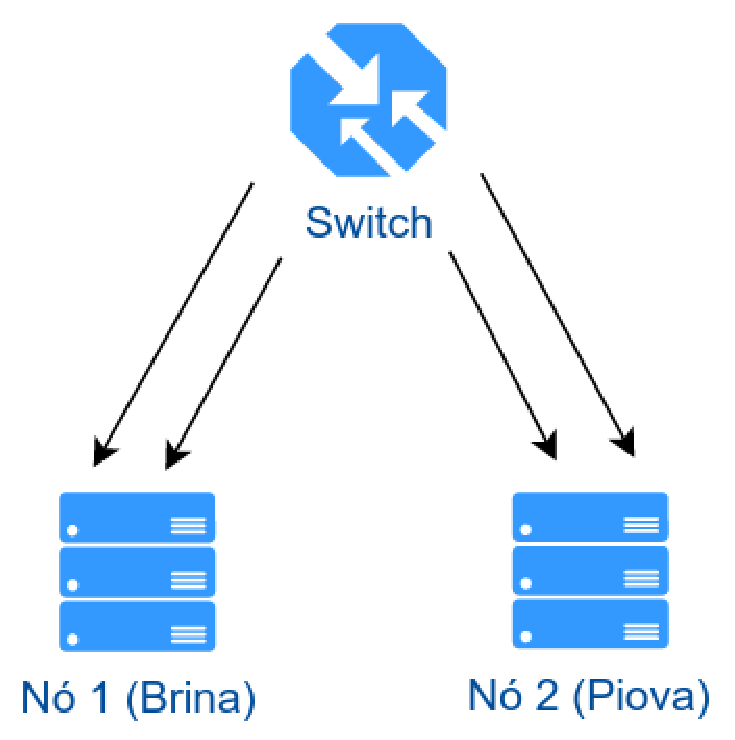
\includegraphics[width=180px]{img/projeto_fisico.eps}
 \caption{Estrutura física.}
 \label{fig:projeto_fisico}
\end{figure}

Para a configuração de rede manteve-se o \textit{link aggregation} e utilizou-se uma \textit{bridge} para incluir as máquinas virtuais à rede.
Os detalhes da configuração estão localizados no Apêndice \ref{ap:confrede}.

Na Figura \ref{fig:servidores_brina_piova} tem-se a imagem dos servidores, o primeiro é o \textit{Brina} (\textit{Dell PowerEdge 2950}), 
e o segundo servidor é o \textit{Piova} (\textit{Dell PowerEdge R410}).

\begin{figure}[h!]
 \centering
 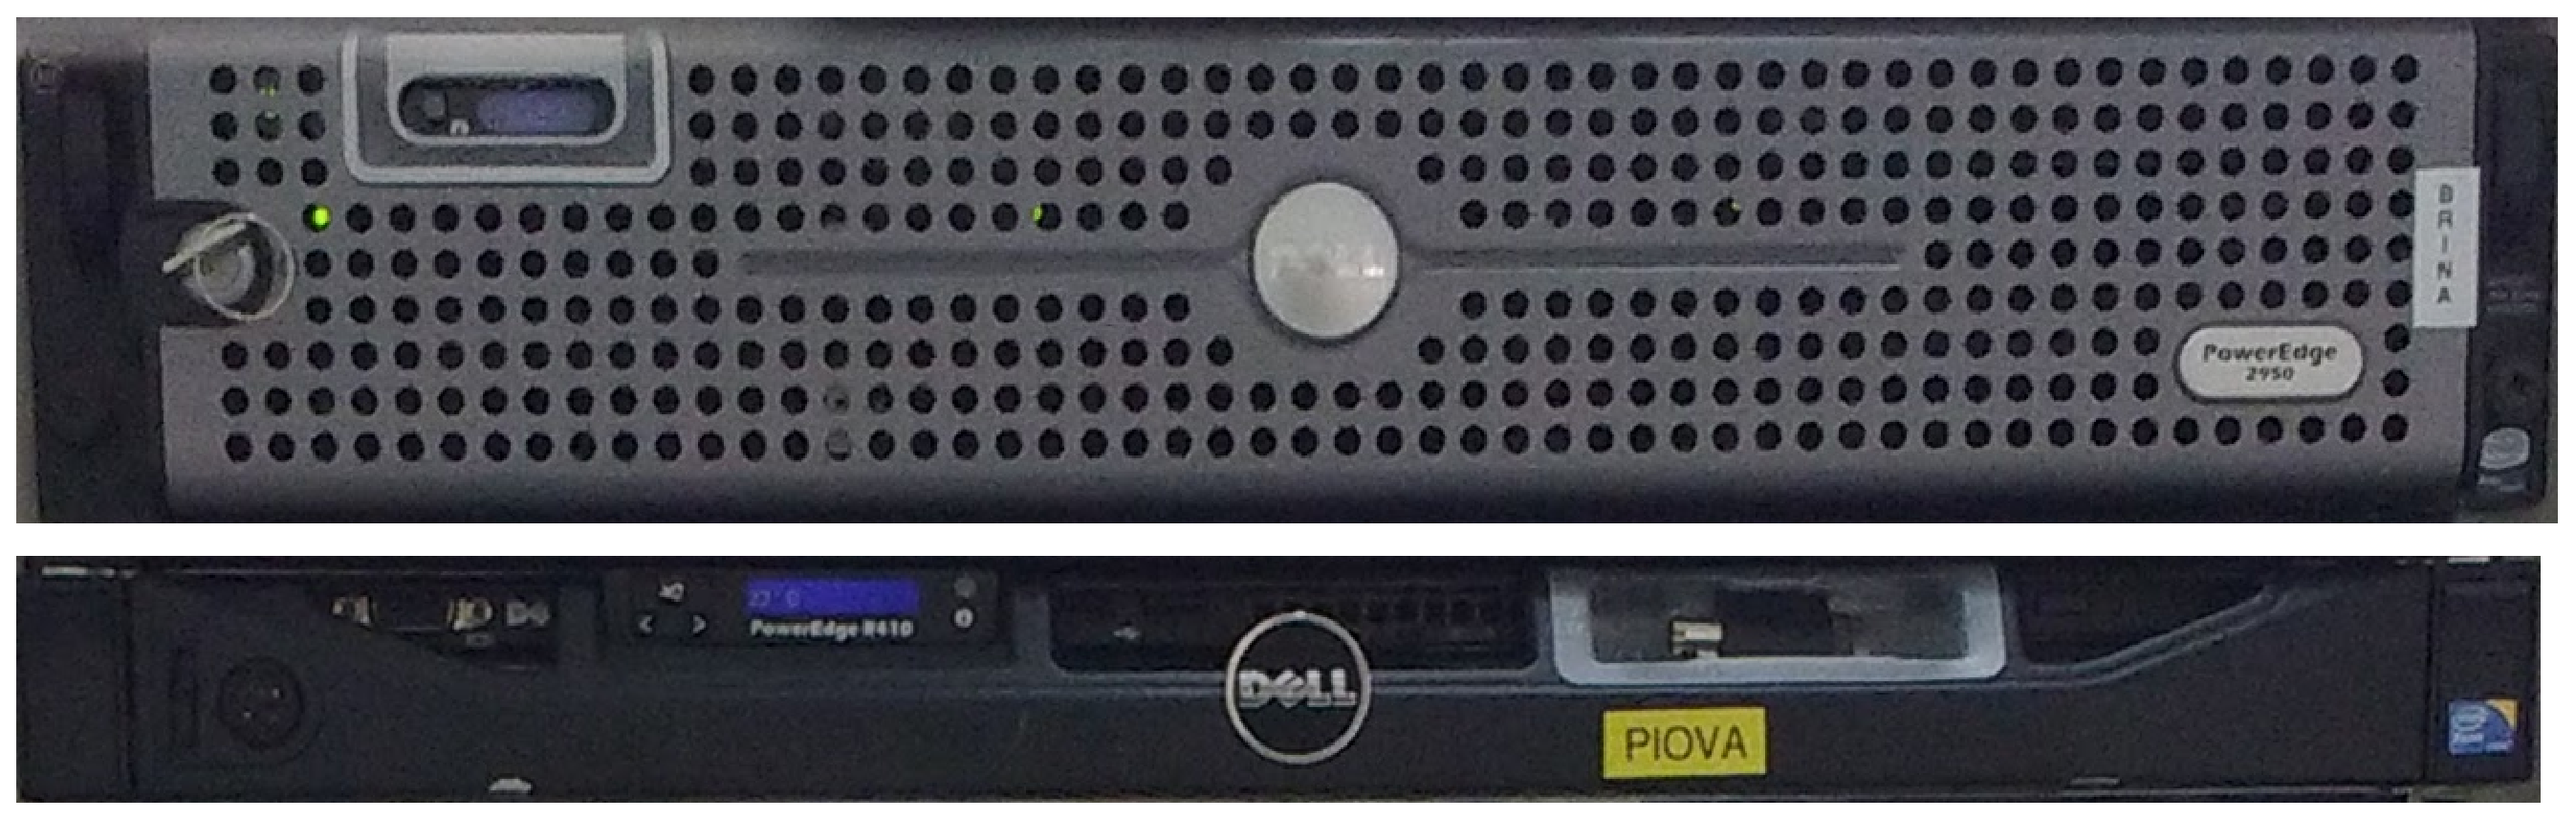
\includegraphics[width=300px]{img/servidores_brina_piova.eps}
 \caption{Servidores.}
 \label{fig:servidores_brina_piova}
\end{figure}

A estrutura lógica dos servidores juntamente com as máquinas virtuais e seus respectivos serviços são apresentados na Figura 
\ref{fig:projeto_estrutura}. Para a replicação de dados foi utilizado o \textit{software} \ac{DRBD}, que foi configurado no modo 
\textit{dual-master} onde os dois nós são configurados como primários. Para tal configuração é necessário utilizar um sistema de arquivos 
distribuídos que faz o gerenciamento do acesso aos dados, o \textit{software} adotado foi o \ac{OCFS2}. 
Os detalhes da instalação e da configuração de disco, \ac{DRBD} e sistema de arquivos estão detalhadas no Apêndice \ref{ap:confdisco}. 
O \textit{software} \textit{Pacemaker} faz o gerenciamento do \textit{cluster}, sendo responsável pela gerência, monitoramento e migração das 
\acp{VM} entre os nós.

\begin{figure}[h!]
 \centering
 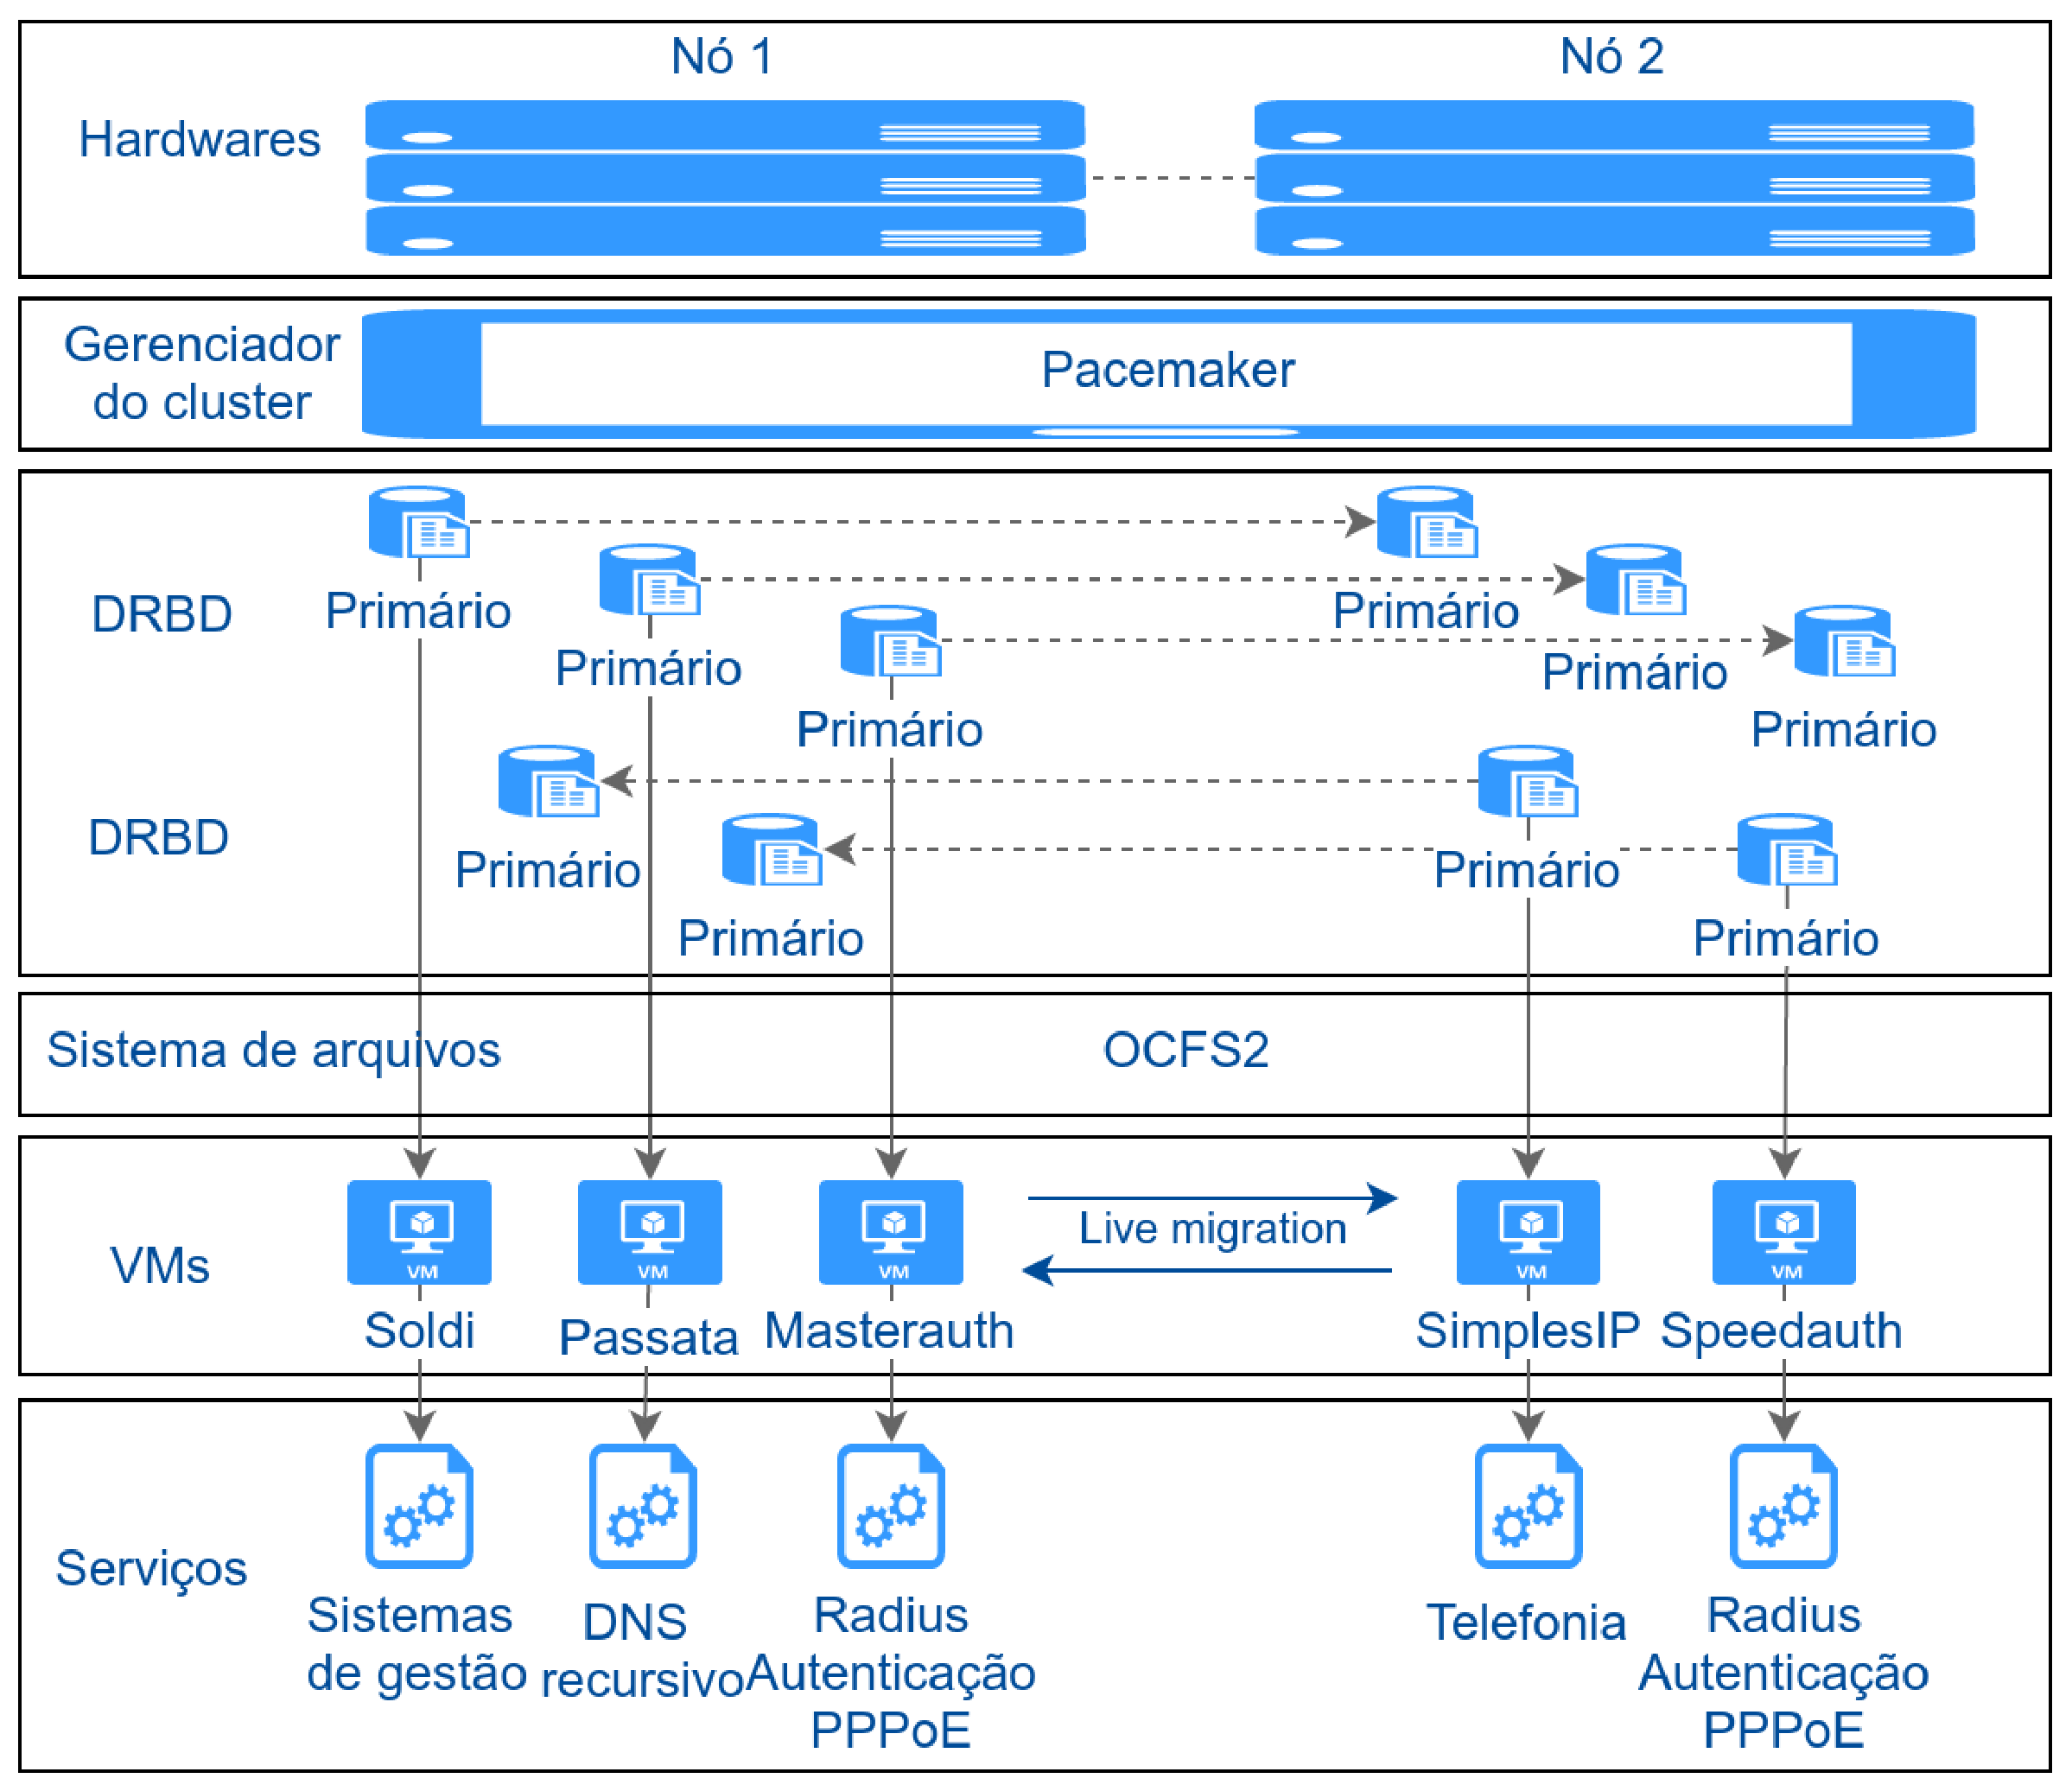
\includegraphics[width=350px]{img/projeto_estrutura.eps}
 \caption{Estrutura do \textit{cluster}.}
 \label{fig:projeto_estrutura}
\end{figure}

%drbd
% O \ac{DRBD} será configurado no modo \textit{master-slave}, sendo que para cada disco das máquinas virtuais será criado um dispositivo de 
% replicação \ac{DRBD}. E para utilizar esse dispositivo como disco de uma máquina virtual será criado um volume lógico 
% \ac{LVM}\footnote{LVM é uma ferramenta de código aberto que possibilita a manipulação de discos rígidos, através da criação de grupos de volumes 
% e volumes lógicos para \textit{Linux}.} \cite{lvm}. 

Deste modo, tem-se o ambiente pronto para a criação das \acp{VM}, sendo assim criou-se uma instância para cada servidor virtual. 
Como pode ser observado no Figura \ref{fig:projeto_estrutura}, criou-se três instâncias no Nó 1 e duas instâncias no outro Nó 2. De fato, o 
primeiro possui as instâncias dos servidores \textit{Soldi}, \textit{Passata} e \textit{Masterauth}. Já o segundo nó possui as instâncias dos 
servidores \textit{SimplesIP} e \textit{Speedauth}. Desta forma, quando houver uma falha em um nó, as instâncias serão iniciadas no nó disponível.
O detalhamento da configuração do \textit{Pacemaker} estão no Apêndice \ref{ap:confpacemaker}.


\section{Validações e testes}
\label{section:testes}

O objetivo desta seção é comprovar que a gerência de falhas é importante para um ambiente computacional, além de destacar que a gerência da 
manutenção também é favorecida por esta implementação.
A metodologia de testes deste trabalho foi fundamentada nos trabalhos de \citet{reis2009} e \citet{goncalves2009}, a mesma foi desenvolvida para 
possibilitar a análise e eficácia do ambiente de alta disponibilidade. 

Os testes desenvolvidos estão detalhados nas próximas seções, neles tem-se a justificativa, a aplicação e os resultados obtidos.
Observa-se que os testes foram efetuados com uma máquina virtual que não possui serviço crítico, pois esses testes possuem risco de perda de dados.
Contudo, na Seção \ref{section:comparacaofinal} será feito uma análise com dados obtidos do ambiente final executando os serviços críticos.

\subsection{Teste 1 - Desligamento físico}
%Desligamento físico (simulação falha de hardware ou eletrica): 4 vezes para medir tempo de downtime dos serviços e dos nodes (servico não crítico)

Este teste faz a simulação de falhas de \textit{hardware} ou falhas elétricas em um nó do \textit{cluster}. Com este teste também pode-se 
validar o processo de \textit{failover} dos serviços (máquinas virtuais) que estavam executando no nó que falhou, bem como medir o tempo de 
indisponibilidade dos serviços.

O procedimento deste teste é o seguinte:
\begin{itemize}
 \item Acessar o terminal do servidor de monitoramento;
 \item Executar comando \textit{ping} e medir o tempo de indisponibilidade (\textit{script} no Apêndice \ref{ap:scriptindisp});
 \item Forçar desligamento do nó;
 \item Aguardar máquinas virtuais inicirem no outro nó;
 \item Finalizar a medição do tempo e \textit{ping}.
\end{itemize}

Este procedimento foi executado 4 vezes para possibilitar o cálculo da média, sendo que este foi aplicado 2 vezes em cada nó. Deste modo, 
criou-se a Tabela \ref{tab:teste1resultadosvirt} a qual possui os dados resultantes dos testes e das medições efetuada sobre a máquina virtual.
% 15/09

\begin{table}[h!]
\caption{Resultados do teste 1 com servidor virtual.}
\label{tab:teste1resultadosvirt}
\begin{center}
\begin{tabular}{|l|p{2.3cm}|p{2.2cm}|p{2.5cm}|p{2cm}|p{2.7cm}|}\hline
 & \textbf{Tempo do teste} & \textbf{Pacotes transmitidos} & \textbf{Percentual de pacotes perdidos} & \textbf{Latência média} & \textbf{Tempo de indisponibilidade} \\\hline
Teste 1 & 299,92 segundos & 301 & 0 & 0,21 ms & 0 segundos \\\hline
Teste 2 & 299,91 segundos & 301 & 0 & 0,22 ms & 0 segundos \\\hline
Teste 3 & 300,15 segundos & 189 & 37 & 7,06 & 86 segundos \\\hline
Teste 4 & 300,49 segundos & 216 & 28 & 4,96 & 76 segundos \\\hline
Média & 300,11 segundos & 251,75 & 16,25 & 3,11 & 40,5 segundos \\\hline
\end{tabular}
\end{center}
\end{table}

Pode-se observar que o tempo de indisponibilidade da máquina virtual é baixo, pois ele é iniciado no outro nó logo após o desligamento do 
primeiro nó. Destaca-se que o \ac{MTTR} seria significativamente maior caso fosse necessário reconfigurar a máquina virtual, reinstalar as 
aplicações, configurá-las e restaurar o \textit{backup}. Dependendo do servidor e da aplicação, a indisponibilidade poderia ser maior que 24 horas.

Na Tabela \ref{tab:teste1resultados} tem-se as médias dos testes dos servidores físicos, pode-se perceber o elevado percentual de pacotes perdidos. 
Além disso, percebe-se a diferença do tempo de indisponibilidade da máquina virtual que é de 40,5 segundos comparado com os servidores 
físicos que são de 169 e 205,5 segundos.

\begin{table}[h!]
\caption{Resultados do teste 1 dos servidores físicos.}
\label{tab:teste1resultados}
\begin{center}
\begin{tabular}{|l|p{2.3cm}|p{2.2cm}|p{2.5cm}|p{2cm}|p{2.7cm}|}\hline
 & \textbf{Tempo do teste} & \textbf{Pacotes transmitidos} & \textbf{Percentual de pacotes perdidos} & \textbf{Latência média} & \textbf{Tempo de indisponibilidade} \\\hline
Média Brina & 300,03 segundos & 300,5 & 58,5 & 20,68 & 169 segundos \\\hline
Média Piova & 300 segundos & 300,5 & 69,5 & 31,44 ms & 205,5 segundos \\\hline
\end{tabular}
\end{center}
\end{table}

A Figura \ref{fig:teste1_disponibilidade} demonstra a disponibilidade dos servidores físicos \textit{Brina} e \textit{Piova} e da máquinas virtual 
\textit{Trapel}. A máquina virtual teve apenas 1 minuto e 10 segundos de \textit{downtime}, deste modo, caso o \textit{hardware} o qual a máquina
virtual está executando falhe o serviço será reestabelecido neste curto período de tempo.

\begin{figure}[h!]
 \centering
 \includegraphics[width=470px]{img/teste1_disponibilidade.eps}
 \caption{Disponibilidade servidores físicos \textit{Brina} e \textit{Piova} e máquinas virtual \textit{Trapel}.}
 \label{fig:teste1_disponibilidade}
\end{figure}


\subsection{Teste 2 - Manutenção agendada}
%Agendamento de manutenção (reboot para atualização de software): 2 semanas ou mais, 1 manutenção por semana, com live migration, reboot e 
%atualizacao de kernel dos nodes. Resultados: latencia, comparacao downtime servidor virtual e fisico, log

Este teste foi criado com intuito de demonstrar que não ocorre indisponibilidade para efetuar manutenções previamente agendadas no ambiente criado.
Reinicializações são necessárias para manutenções de \textit{hardware}, atualização de \textit{software} e até mesmo para rejuvenescimento de
\textit{software} \cite{melo2014}.

O procedimento deste teste é o seguinte:
\begin{itemize}
 \item Executar comando \textit{ping} e medir o tempo de indisponibilidade (\textit{script} no Apêndice \ref{ap:scriptindisp});
 \item Executar o \textit{script} que desativa o nó (comando \textit{standby}) e executa o \textit{reboot} (Apêndice \ref{ap:scriptmanutencao});
 \item Após retorno do nó executar novamente o \textit{script} anterior para retorno do nó ao \textit{cluster};
 \item Finalizar a medição do tempo e \textit{ping}.
\end{itemize}

Este roteiro foi executado 2 vezes por semana em cada nó, durante 2 semanas. Para sua execução dos \textit{scripts} foi utilizada a ferramenta 
\textit{crontab} do \textit{Linux}. Com os dados obtidos criou-se a Tabela \ref{tab:teste2resultados}.
% 17/09 a 30/09
% crontab brina:
% */10 04 * * 2 /usr/local/sbin/script_pacemaker_manutencao.sh
% crontab piova:
% */10 04 * * 4 /usr/local/sbin/script_pacemaker_manutencao.sh
% crontab monit:
%59 03 * * 2 cd /home/bruno/pacemaker/teste2/; bash indisponibilidade.sh 186.195.16.14 3
%59 03 * * 2 cd /home/bruno/pacemaker/teste2/; bash indisponibilidade.sh 186.195.16.13 3
%59 03 * * 4 cd /home/bruno/pacemaker/teste2/; bash indisponibilidade.sh 186.195.16.6 2
%59 03 * * 4 cd /home/bruno/pacemaker/teste2/; bash indisponibilidade.sh 186.195.16.13 2


\begin{table}[h!]
\caption{Resultados do teste 2.}
\label{tab:teste2resultados}
\begin{center}
\begin{tabular}{|l|p{2.2cm}|p{2.5cm}|p{2.5cm}|p{1.5cm}|p{3cm}|}\hline
\textbf{Tipo} & \textbf{Média do tempo do teste} & \textbf{Média dos pacotes transmitidos} & \textbf{Média do percentual de pacotes perdidos} & \textbf{Latência média} & \textbf{Média do tempo de indisponibilidade} \\\hline
Brina & & & & & \\\hline
Piova & & & & & \\\hline
Servidor virtual & & & & & \\\hline
\end{tabular}
\end{center}
\end{table}

%Pode-se observar que não houve \textit{downtime} na máquina virtual, e consequentemente nos serviços.
%Porém, tem-se uma latência maior durante o processo de \textit{live migration}, como pode ser observado na Figura X.
...

grafico latencia

%grafico comparativo nagios da disponibilidade do servidor fisico e do virtual
%grafico nagios - Trends(grafico) ou Availability (resumo) - Hosts - servidor - tempo 17/09 a 30/09 + Include Soft States = yes
A Figura X demonstra a disponibilidade da máquina virtual (a) e dos nós (b), esses dados foram retirados da ferramenta de monitoramento da empresa,
\textit{Nagios}. Comparando os gráficos pode-se perceber a diferença do \textit{uptime} entre servidores físicos e o virtual.
%%figura
...

%log do pacemaker
O processo de \textit{standby} feito pelo \textit{Pacemaker} está detalhado no \textit{log} abaixo:
...

\subsection{Teste 3 - Desligamento por software}
%Desligamento por software (reboot manual): 4 vezes para medir tempo de downtime dos servicos e dos nodes (servico nao critico)
%simulação de falha de software ou manutenção emergencial

Esse teste simula falhas de \textit{software} nos nós do \textit{cluster}, como por exemplo do \textit{software} de virtualização. Esse tipo de 
situação também pode ser necessário em uma manutenção emergencial, onde, por exemplo, é preciso desligar o servidor.

O procedimento deste teste é o seguinte:
\begin{itemize}
 \item Acessar o terminal do servidor de monitoramento;
 \item Executar comando \textit{ping} e medir o tempo de indisponibilidade (\textit{script} no Apêndice \ref{ap:scriptindisp});
 \item Acessar o terminal do nó que será reiniciado;
 \item Executar o comando \textit{reboot};
 \item Aguardar máquinas virtuais inicirem no outro nó e aguardar retorno do nó reiniciado;
 \item Finalizar a medição do tempo e \textit{ping}.
\end{itemize}

O procedimento deste teste foi executado 4 vezes no total, sendo que foram executadas 2 vezes em cada nó. A Tabela \ref{tab:teste3resultados}
demonstra os dados do servidor físico e do virtual.
% 09/09

\begin{table}[h!]
\caption{Resultados do teste 3.}
\label{tab:teste3resultados}
\begin{center}
\begin{tabular}{|l|p{2.2cm}|p{2.5cm}|p{2.5cm}|p{1.5cm}|p{3cm}|}\hline
\textbf{Tipo} & \textbf{Média do tempo do teste} & \textbf{Média dos pacotes transmitidos} & \textbf{Média do percentual de pacotes perdidos} & \textbf{Latência média} & \textbf{Média do tempo de indisponibilidade} \\\hline
Servidores físicos & 260,53 segundos & 261 & 60,75 & 14,98 ms & 152,75 segundos \\\hline
Servidor virtual & 156,98 segundos & 158 & 18,75 & 0,2217 ms & 5 segundos \\\hline
\end{tabular}
\end{center}
\end{table}

Pode-se observar que o tempo de indisponibilidade do servidor virtual é consideravelmente menor que o tempo do servidor físico, ele representa 
apenas 3,27\% do tempo de indisponibilidade do servidor físico. Além disso, pode-se perceber que o percentual de perda de pacotes é menor.
Este teste pode ser comparado com um caso que ocorreu a alguns meses na empresa, um servidor de virtualização, que é atualizado de forma automática,
foi reiniciado, porém ocorreu um erro na atualização e o servidor não pôde iniciar corretamente. Os serviços executados nele ficaram 
aproximadamente 6 horas indisponíveis.

\subsection{Comparação final da disponibilidade}
\label{section:comparacaofinal}
%Medição da disponibilidade dos serviços críticos por 1 mes (outubro) e comparar ao mês de setembro no ambiente antigo com 
%uma Reinicialização dos servidores físicos (reiniciados em 06/09/16)

Como já mencionado anteriormente, esta seção analisará os serviços críticos no ambiente final de produção que possui as máquinas virtuais
definidas na Seção \ref{section:maqservcrit}. 
%...foi mensurado a disponibilidade

adicinar gráficos de disponibilidade final dos serviços críticos:

%Medição através do comando ping e do Nagios, que utiliza ping para calcular o tempo de downtime
%Tabela com perda de pacotes, latencia, tempo de indisponibilidade X node fisico e maquina virtual

